\documentclass[11pt, oneside]{article} 
\usepackage{geometry}
\geometry{letterpaper} 
\usepackage{graphicx}
	
\usepackage{amssymb}
\usepackage{amsmath}
\usepackage{parskip}
\usepackage{color}
\usepackage{hyperref}

\graphicspath{{/Users/telliott/Github/precalculus/fig/}}

\title{Basic algebra}
\date{}

\begin{document}
\maketitle
\Large

There is very little algebra that needs to be memorized for where we're going.  We just finished a chapter about the sum of integer squares.  If you can follow that, you're in good shape.  If not, go back and work through it again, carefully.

Here is a bit more:

\subsection*{inequality}
You have surely seen and used the symbols $>$ (greater than), and $<$ (less than) before we used them a second ago.

Among the axioms of the number systems is the collection of \emph{order axioms}.  A few definitions:

$\bullet$ \ $x < y$ means that $y - x$ is positive

$\bullet$ \ $y > x$ means that $x < y$

For arbitrary numbers $a$ and $b$ only one of three statements is true:  

$\bullet$ \ $a < b$

$\bullet$ \ $a = b$

$\bullet$ \ $a > b$

There is no attempt or need to be systematic here.  Let us just mention that these properties (and their kin) are true not just for natural numbers, but also for the rational numbers and the real numbers, as we will see in due course.  

Here are a few important theorems about order which we will use often:

$\bullet$ \ If $a < b$, and $c$ is any number, then $a + c < b + c$

$\bullet$ \ If $a < b$, then $-b < -a$

$\bullet$ \ If $a < b$ and $c > 0$, then $ac < bc$

The first one above implies the second and the third.

\subsection*{algebraic operations}

$\bullet$ addition:  $a + b$

$\bullet$ subtraction:  $a - b = a + (-b)$

The negative integers and $0$ solve the problem of how to evaluate $a - b$ when $b \ge a$.

$\bullet$ multiplication:  $a \cdot b$, also often written $ab$ (but not $a \times b$, at this level).

And then:

$\bullet$ division $a/b$, equivalent to finding a number $c$ such that $c \cdot b = a$.

\subsection*{algebra}
As you know, the basic axioms of algebra include the following:

$\bullet$ \ Commutativity for addition and multiplication: 
\[ a + b = b + a, \ \ \ \ \ \ a \cdot b = b \cdot a \]

$\bullet$ \  Associativity for addition and multiplication:
\[ (a + b) + c = a + (b + c), \ \ \ \ \ \ (a \cdot b) \cdot c = a \cdot (b \cdot c) \]

$\bullet$ \ Distributivity of addition over multiplication:  
\[ a \cdot (b + c) = a \cdot b + a \cdot c \]

$\bullet$ \ Additive identity:  $0 + a = a$.

$\bullet$ \ Multiplicative identity:  $1 \cdot a = a$.

\subsection*{binomial theorem}

One basic idea from algebra is the binomial theorem:
\[ (a + b)^2 = (a + b)(a + b) = a^2 + 2ab + b^2 \]
so then
\[ (a + b)^3 = (a + b)(a^2 + 2ab + b^2) \]
\[ = a^3 + 3a^2b + 3ab^2 + b^3 \]
And in general, to get the next $n+1$ power, go through the expansion for the $n$ power and multiply each term separately by $a$ and $b$.

You will find that the cofactors are given by Pascal's triangle.

\begin{center} 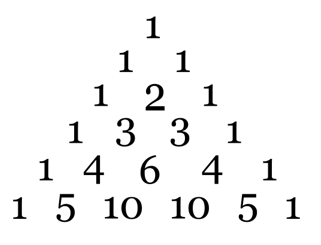
\includegraphics [scale=0.45] {pascal.png} \end{center}

\[ (a + b)^3 = a^3 + 3a^2b + 3ab^2 + b^3 \]
\[ (a + b)^4 = a^4 + 4a^3b + 6a^2b^2 +  4 ab^3 + b^4 \]
\[ (a + b)^5 = a^5 + 5a^4b + 10a^3b^2 + 10a^2b^3 +  5 ab^4 + b^5 \]
\[ \dots \]

If you substitute $-b$ for $b$ you will find that everything is exactly the same, except those terms with $b$ raised to an odd power have acquired a minus sign.
\[ (a - b)^3 = a^3 - 3a^2b + 3ab^2 - b^3 \]

Hence
\[ (a-b)(a^2 - 2ab + b^2) = a^3 - 3a^2b + 3ab^2 - b^3 \]

The binomial theorem is usually stated and worked with in terms of positive integers.  

But it actually works for negative integers and fractional powers as well.  The big difference is that the series of terms is \emph{infinite}.

Newton discovered that, though he didn't prove it.  He just used it as a tool.  He found that

\[ \frac{1}{1 + x} = (1+x)^{-1} \]
\[ = 1 - x + x^2 - x^3 + x^4 + \cdots  \]

Newton checked this by multiplying:
\[ (1+x)(1 - x + x^2 - x^3 + x^4 + \cdots) \]
\[ = 1 - x + x^2 - x^3 + x^4 + \cdots \]
\[ \ \ \ \ \ \ \ + x - x^2 + x^3 - x^4 + \dots = 1  \]

But be careful!  What happens if $x = -1$?

\subsection*{factoring}
Here's something we will use often:  the difference of two squares.
\[ a^2 - b^2 = (a + b)(a - b) \]

The classic quadratic equation is often written
\[ y = ax^2 + bx + c \]
This is a parabola that opens up ($a > 0$).  

Depending on the values of the \emph{coefficients} $a,b,c$, this equation may or may not have solutions when $y = 0$
\[ ax^2 + bx + c = 0 \]
\[ x^2 + \frac{b}{a}x + \frac{c}{a} = 0 \]

Suppose that $r$ and $s$ are such solutions, then 
\[ (x - r)(x - s) = 0 \]
and so
\[ x^2 - (r + s)x + rs = 0 \]
A fair amount of effort in algebra goes into guessing values of $r$ and $s$ that work, that have the appropriate sum and difference to match the equation we are given.

However, the answers frequently are not integers, and in that case, this approach is doomed.  

A formula that always works is the quadratic formula:
\[ x = \frac{-b \pm \sqrt{b^2 - 4ac}}{2a} \]

I said "always works".  To be more precise, it works if there are any solutions.  If the discriminant $D = b^2 - 4ac$ is negative, then we're trying to take a square root of a negative number, and we don't know how to do that in the real numbers.

We will develop this more in the chapters on analytic geometry.  That's really all you will need.



\end{document}